\documentclass[10pt,twocolumn,letterpaper]{article}
  \usepackage[utf8]{inputenc}  
  \usepackage{cvpr}
  \usepackage{times}
  \usepackage{epsfig}
  \usepackage{graphicx}
  \usepackage{amsmath}
  \usepackage{amssymb}
  
  \usepackage{float}

  % Include other packages here, before hyperref.
  
  % If you comment hyperref and then uncomment it, you should delete
  % egpaper.aux before re-running latex.  (Or just hit 'q' on the first latex
  % run, let it finish, and you should be clear).
  \usepackage[breaklinks=true,bookmarks=false]{hyperref}
  
  \cvprfinalcopy % *** Uncomment this line for the final submission
  
  %\def\cvprPaperID{****} % *** Enter the CVPR Paper ID here
  \def\httilde{\mbox{\tt\raisebox{-.5ex}{\symbol{126}}}}
  
  % Pages are numbered in submission mode, and unnumbered in camera-ready
  %\ifcvprfinal\pagestyle{empty}\fi
  \setcounter{page}{1}
  \begin{document}
  
  %%%%%%%%% TITLE
  \title{Sin City, Classification of Regional Songs in Turkey}
  
  \author{Muhammet Emin Özgür\\
  %Institution1 address\\
  {\tt\small b21427229@cs.hacettepe.edu.tr}
  % For a paper whose authors are all at the same institution,
  % omit the following lines up until the closing ``}''.
  % Additional authors and addresses can be added with ``\and'',
  % just like the second author.
  % To save space, use either the email address or home page, not both
  \and
  Ufuk Umut Şentürk\\
  %First line of institution2 address\\
  {\tt\small b21427435@cs.hacettepe.edu.tr} \\
  \and
  Muazzez Şule Karaşlar\\
  %First line of institution2 address\\
  {\tt\small b21427066@cs.hacettepe.edu.tr}\\
  {Machine Learning Lab, Department of Computer Engineering}\\
  {Hacettepe University, Ankara, TURKEY}\\
  }
  
  \maketitle
  %\thispagestyle{empty}
  %%%%%%%%% ABSTRACT
  \begin{abstract}
    In most cultures we can define a generic type of songs that defines the culture. We can even pinpoint the differences between similar cultures but relatively in a different region which might be city, county or state. This is the point where idea came to classify folk songs in Turkey region by region. This paper discusses methods of studying the region style classification of Turkish folk songs with CNN(Convolutional Neural Network), SVM(Support Vector Machine), K-NN(K Nearest Neighbor). According to geographical region of Turkey, we have classified Turkish folk songs into 7 regions which can be seen
    as cultural regions., and used 917 Turkish folk songs in our experiment. Thus, those regions do not have completely different cultures,but differences are visible which one of them is the regional songs. For instance, tulum, kemençe(endemic musical instruments for Karadeniz) can be heard in Karadeniz songs which are distinguishable from other regions songs. However, some regions have same musical infrastructure which are rhythm, instruments, chords or notes patterns and vocal type which is hard to distinguish for a human being. This one is probably the hardest challenge we faced. Hence, feature extraction was the crucial point for this matter. After gathering our dataset from youtube which is not good idea and convert them aau, m4a and ogg formats features have been extracted from audio files of the songs that are melspectogram, MFCC(Melfrequency cepstral coefficients), Spectral centroid ,Spectral roll-of, Zero-crossing rate. Those are the features we used for our classification. We used CNN, SVM and KNN as our models, but in the prediction part we use voting system for that song .
  \end{abstract}
  %%%%%%%%% BODY TEXT
  \section{Introduction}
  \paragraph{}In machine learning most important step is the feature extraction. Just by improving features will increase dramatically for contemporary machine learning models. In the audio feature extraction, current state-of-art is being provided by MIR(Music Information Retrieval) research field. MIR is a huge field that has been under the spotlight since Tzanetakis and Cook released a paper on Music Genre Classification in 2002\cite{genre_classification_tp}. MIR includes audio feature extraction, signal processing, audio analyse etc. Audio feature extraction is what we are interested in MIR research field. We are planning mainly to use features: Chroma-gram, MFCC(Mel-frequency cepstral coefficients), Spectral centroid, Spectral roll-of, Zero-crossing rate, etc. We will also use other features for reference points but these will be the main features.
  Machine learning model selection for the job is not without importance. State-of-art models are plentiful, however they are mostly specific for a given problem. In order to find the best classification, we will use various models which will be CNN(Convolutional Neural Network), SVM(Support Vector Machine), K-NN(K Nearest Neighbor). These machine learning models will be implemented with various contemporary features discussed in MIR. Subsequently these will be analysed.   
  Analyzing will be last step in our paper. We will gather results after the testing which in a matrix as rows for machine learning models and columns for features. Best model and features will be apparent after the testing is done. Confusion matrix will be constructed by using our best model and features.   
  
  %-------------------------------------------------------------------------
  \section{Related Works}
  
  \paragraph{}In this paper, classification problem is more specific than any other work. since Tzanetakis and Cook presented music genre classification\cite{genre_classification_tp}, a lot of work has been done. 
  For Audio processing and analyzing, it is hard to build-up a reliable feature extractor system for audio seems to be a more challenging task than classification problem.
  For this purpose some researches have been done about features extraction such as; MFCC\cite{mffc}, Chromogram\cite{chroma}, Zero-crossing rate, Spectral-Centroid\cite{spectral_centroid}.
  \paragraph{}The most known study for folk song classification which is based on region has been done for China. On paper in interest, 74 features have been extracted from audio files of the songs, and classified by an audio classifier on SVM which is one of our concern. Research shows usthat SVM without feature selection is a very effective classification method with the combination of 13-dimension MFCC and 10-dimension without feature selection. It points us to post processing and segmentation plays key role in here. Other research is called "Regional Classification of Traditional Japanese Folk Songs" by Akihiro KAWASE, Akifumi TOKOSUMI has been made. That research use music corpora consisting of 202,246 tones from 1,794 song pieces from 45 prefectures in Japan which is big enough.
  
  \paragraph{}In another research\cite{feature_extraction_automatic_cnn}, presented a methodology to automatically extract musical patterns features from audio music using the CNN which is easy to use for feature extractors, it because need minimal prior knowledge to construct. Some other paper uses\cite{genre_classification} various machine learning algorithms that are including k-nearest neighbor (kNN), k-means, multi-class SVM, and neural networks to classify the following four genres: classical, jazz, metal, and pop and only Mel Frequency Cepstral Coefficients (MFCC) is used to characterize data.
  Using CNN is become quite popular in other ML fields with each other. Qiuqiang Kong, et al\cite{genre_cnn} stated that many manual-selected features such as MFCC have been applied to music processing but they are not effective for music genre classification. In their work, it is presented an algorithm based on spectrogram and CNN and compared with MFCC, the spectrogram contains more details of music components such as pitch, flux, etc. 
  
  \paragraph{}By the nature of data involved in analysis, the field of music genre classification is divided to two different scopes: symbolic and audio. Symbolic music genre classification studies songs in their symbolic format, such as MIDI, MusicXML, etc. Various models (Basili et. al. \cite{to_basili}, McKay et. al. \cite{to_mckay}, Ponce et. al. \cite{to_ponce}) have been proposed to perform symbolic music genre classification. Feature sets representing instrumentation, musical texture, rhythm, dynamics, pitch statistics, melody, etc. are used as input for a wide variety of generic multi-class classifiers.

  \paragraph{}Fiebrink and Fujinaga \cite{to_fiebrink} discuss the use of complex feature representation and the necessary computational resources to compute them. They have employed 74 low-level features available at the jAudio \cite{to_jaudio}. jAudio is a software package for extracting features from audio files as well as for iteratively developing and sharing new features. Then, these features can be used in many areas of music information retrieval (MIR) research. To evaluate feature selection in the AMGC problem they have employed a forward feature selection (FFS) procedure and also a principal component analysis (PCA) procedure. The experiments were carried out using the Magnatune database (4,476 music pieces from 24 genres) \cite{magnatune} and the results over a testing set indicate that accuracy rises from 61.2\% without feature selection to 69.8\% with FFS and 71\% with PCA.

  \paragraph{}Yaslan and Cataltepe \cite{to_yaslan} have also employed a feature selection approach for music genre classification using search methods, such as forward feature selection (FFS) and backward feature selection (BFS). FFS and BFS methods are based on a guided search in the feature space, starting from an empty set and from the entire set of features, respectively. Several classifiers were used in the experiments such as linear and quadratic discriminant classifiers, Naive-Bayes, and variations of the k-NN classifier. They have employed the GTZAN database and the MARSYAS framework for feature extraction \cite{genre_classification_tp}. The experimental results have shown that feature selection, the use of different classifiers, and a subsequent combination of results can improve the music genre classification accuracy.

  \paragraph{}Bergstra et al. \cite{to_bergstra} use AdaBoost which performs the classification iteratively by combining the weighted votes of several weak learners. The feature vectors were built from several features like fast Fourier transform coefficients, real cepstral coefficients, MFCCs, zero-crossing rate, spectral spread, centroid, roll-off and autoregression coefficients. Experiments were conducted considering the music genre identification task and the artist identification task of the 2005 Music Information Retrieval EXchange competition (MIREX’05). The proposed ensemble approach have shown to be effective in three music genre databases. The best accuracies in the case of the music genre identification problem vary from 75.10\% to 86.92\%. This result allowed the authors to win the task of music genre identification in the MIREX’05 competition.

  \paragraph{}Nearly all approaches are used in this manner, Keunwoo et al.\cite{crnn_for_ml} had used Convolutional Recurrent Neural Network. Another paper focused on music recommendation  by using CNN with ReLU activation function with pre-processed MFCC spectograms\cite{cnn_recommendation}. Many more paper has been written for this purpose. However, most of them suggest to use MFCC and melspectrogram for feature extraction or pre-processing part which has been done by us.
  %-------------------------------------------------------------------------
  
  \section{Methodology}
  
  \subsection{Data Set}
  \paragraph{}We have gathered our data from youtube playlist. There are various regional playlist which we have found with quick search\cite{data_set}. We obtained these in ogg format and as smallest bitrate as possible we can find in order to save space. JDownloader\cite{jdownloader} used to download these playlist with ease.  JDownloader take care of everything related to downloads, from the beginning till the end. There is no need neither to download each link separately nor to be aware of any countdown or waiting time . All we have to do to download files with JDownloader is simply copy the link of the file we want to download and this program will detect it instantly, starting the task in a few seconds .Each downloaded audio file is placed in respective folder for label in their classification. In these playlist there might be noise
  such as given song might not be in that region as suggested in the name of the playlist or one song place in more than one playlist which is a rare case. These will be most likely a miniscule noise. Moreover we will add more songs in the
  data set, hence the noise will be smaller with each growth of the data set.Our dataset contains 917 songs .They are placed in 7 folder which is our label number at the same time.They are Aegean, Black Sea, Marmara and Mediterranean ,Central, Eastern and Southeastern Anatolia. All these audio files have size of 1.54 GB.
  
  \subsection{Features}
  \paragraph{}As hitherto cited, MFFC, Spectral Centroid, Spectral roll-of, Zero-crossing rate\cite{genre_classification_tp} are main focus in this paper. Librosa\cite{librosa} is used for feature extraction library. It is not the fastest library, it is only used because of convenience. These features will have tremendous dimension space which would need dimension reduction with PCA(Principle Component Analysis) and feature selection techniques. 
  \begin{figure}[t]
    \begin{center}
    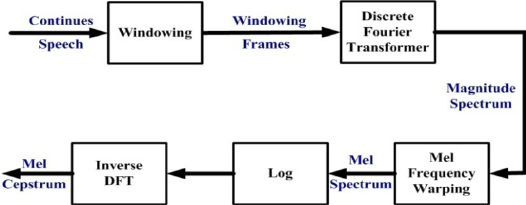
\includegraphics[width=0.8\linewidth]{images/mfcc_calc.png}
    \end{center}  
       \caption{MFCC Calculation Process.\cite{mfcc_calc}}
    \label{fig:mffc}
    \label{fig:onecol}
  \end{figure}
  \paragraph{} Above Figure 1. shows us the calculation steps of MFCC\cite{mfcc_calc}. MFCC is a convenient feature used in speak recognition, signal processing. Alternatively, spectral centroid feature is proposed and used widely. Below figure shows spectral centroid.\cite{spec_centroid}
  \begin{figure}[t]
    \begin{center}
    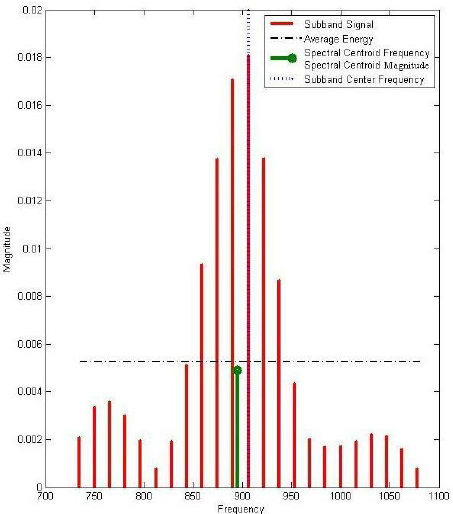
\includegraphics[width=0.8\linewidth]{images/spec_centroid.png}
    \end{center}  
       \caption{Subband signal, average energy, spectral centroid frequency and spectral centroid\cite{spec_centroid}.}
    \label{fig:mffc}
    \label{fig:onecol}
  \end{figure} 
  
  \paragraph{}Zero Crossing Rate is widely used in audio classification. It is time domain feature in the processing window as shown in below
  $$ZCR=\frac{1}{M-1}\sum_{m=0}^{M-1} |sign(x(m)) - sign(x(m-1))|$$
  
  where sign is 1 for positive arguments and 0 for negative arguments, M is the total number of samples in a processing window and $x(m)$ is the value of the $mth$ sample. The algorithm is very simple and used for speech/music classification\cite{speech_music}, genre classification and many more \cite{genre_classification_tp}.
  
  \paragraph{} Speech consists of voiced and unvoiced sounds. The ZCR correlate with the frequency content of a signal, Hence, voiced and unvoiced sounds have low respectively, high zero crossing rates. This results in a high variation of ZCR. Music does not have this variation in ZCR but it has to be said that some pop songs can have high variations in ZCR values.
  
  \paragraph{} Spectral centroid feature is to classify between noise, speech and music. Also\cite{speech_music} it has been used for genre classification. Spectrum centroid is based on analysis of the frequency spectrum of the signal. The frequency spectrum , for use in this feature and several others, us calculated with discrete Fourier transform(DFT). Spectrum centroid is a measure that signifies if the spectrum contains a majority of high or low frequencies. This is correlates with a major perceptual dimension of timbre such as sharpness.
  
  \paragraph{}Li\cite{pattern_letters} used a feature named spectral roll-off frequency (SRF) to classify between noise, speech and music. Its equation is shown below;
  $$SRF(n) = max(h|\sum_{k=0}{h}A(n, k)<TH.\sum_{k=0}{K-1}|A(n, k)|^2)$$
  
  where N is the total number of frames, K is the order of the DFT, TH is a threshold set to 0.92(or something around that value) and $A(n,k)$ is the DFT of the nth frame of a signal and is calculated as shown below. That is, the spectral roll-off frequency is a metric of how high in the frequency spectrum a certain part of the energy lies. The serf is an effective feature for classification between speech and music. The characteristics of an speech signals tend to have lower SRF than music. Music signals contain higher frequencies from instrument as flutes, distortion guitars and ho-hats of the drum. This result in that music signals tend to have high values of SRF. 
  
  \paragraph{}Spectral features are directly computed on the magnitude spectrum and attempt to summarize information about the general characteristics of the distribution of energy across frequencies.The zero-crossing rate is the rate of sign-changes along a signal, i.e., the rate at which the signal changes from positive to negative or back.
  The spectral roll-off is defined as the frequency Rn below which 85\% (usually) of the energy distribution of the magnitude spectrum is concentrated. The spectral centroid is a measure used in digital signal processing to characterize a spectrum. It indicates where the "center of mass" of the spectrum is located. Melspectrogram, spectrum is filtered with Nd different band-pass filters and the power of each frequency band is computed. The mel frequency cepstral coefficients (MFCCs) of a signal are a small set of features (usually about 10-20) which concisely describe the overall shape of a spectral envelope. In MIR, it is often used to describe timbre. Rest of the steps after the discrete Fourier Transform, is meant to mimic human perception.\cite{content_descriptor}
  
  \begin{figure}[t]
    \begin{center}
    \includegraphics[width=1.15\linewidth]{images/mel.png}
    \end{center}  
       \caption{Above figure captions melspectogram feature of one of the 63 part in a song in the training set.}
    \label{fig:mffc}
    \label{fig:onecol}
  \end{figure} 
  \paragraph{}When we look at the characteristics of the features, mel-spectogram and MFCC are best fit for our purpose which we will explain later in this paper. 
  
  \subsection{The Approach}
  \paragraph{}Different approaches, classifiers, data-sets have been tried to get right choice. First of all, features were picked which would be used later as any machine learning problem. As the related works mention MFCC, melspectrogram and spectral features were picked and extracted from songs by librosa library. Library in interest is not enough for long duration signals because it does support short duration songs. That's why it takes so much time even feature extracting part. Thus, we tried different techniques for this job. Initially, we tried to load all the songs and try to extract different features from them. However, songs are not fixed size, one song load time is like 15-20 seconds and eventually RAM cannot stand anymore. Our second approach is extracting features in 30 seconds parts. However, it was not efficient, too. Because librosa loads audio as 22050 Hz which returns 22050*duration\_of\_song that is 661500 elements vector for 30 seconds. After several attempts, our last approach was taking first 30 seconds of song, which gives good results in this paper cite to thirty seconds, split each 30 seconds into 41 or any parametric overlapping frames, one for each of the 60 or any parametric value mel-bands which gives us 60 rows and 41 columns which is an example of data augmentation that is creating several training examples from a single source recording. In our case it makes about 44000 samples from 900 songs. That was way we extracted our mel-spectogram features, and other features could be extracted same way. We also tried other features as another input channels such as delta values of features on the channel one of the input. Also, StandarScalar is used to standardize features by removing the mean and scaling to unit variance. Standardization of a dataset is a common requirement for many machine learning estimators: they might behave badly if the individual feature do not more or less look like standard normally distributed data. Other than that, we saved features as numpy arrays as batches to the disk to relieve RAM usage and time which affected so much in a good way. Because, whole feature array occupies about 800 MB of disk space.
  
  \paragraph{}KNN, SVM and CNN classifiers are used for this project. SVM and KNN is implemented by scikit-learn python-module. We used keras with tensorflow backend for CNN implementation. In implementation detail, we try to design our project according to OOP and modularity rules. We implemented abstract base classifier as super class to other models and we could use inheritance abilities of python which reduced number of code line so much. At the same time, we could implement another classifiers easily with this strategy. For instance, before we changed our feature extraction method, our CNN model could not fit because of RAM, too. That is why, we implemented basic fully connected Neural Network by using keras to see how it ended up with features and that was pretty fast to implement. 
  
  \paragraph{} Lack of RAM and lack of NVDIA card, we could fit our model on GPU with keras if we had one which would speed up whole project process time, forced us to use batch learning. CNN supports that kind of learning natively, but KNN does not so we had to keep whole feature array on the disk. LinearSVM does not support in sci-kit library. Thus, we used SGDClassifier from scikit-learn library which uses Stochastic Gradient Descent (SGD) with linear classifiers such as SVM, logistic regression etc. This estimator implements regularized linear models with SGD learning: the gradient of the loss is estimated each sample at a time and the model is updated along the way with a decreasing strength schedule (aka learning rate). SGD allows minibatch (online/out-of-core) learning with partial\_fit method. We could as SVM classifier this model by picking loss function as a 'hinge' and regularization term as 'l2' and also we could use SGD abilities such as epoch number, learning rate, etc. 
  
  \paragraph{} Before explaining our CNN model, our basic approach was using some kind of voting system with those models for our prediction method. Firstly, songs were splited as you remembered. In the case of 30 seconds part with 41 overlapping frames, 60 mel-band, we had about 63 parts from only one song. Thus, the most predicted label is picked for that song with its possibility. For instance, 53 parts are predicted as 'ege', label 'ege' would be picked with possibility $53/60$ for that song. Those possibilities are needed because of our voting system. After whole models predicted songs, algorithm averages possibilities of same songs that has same label from different models.That average probability is vote number of that label for the song. Say, if we have 3 models and first model predicts first song as 'ege' with 30\% probability, second model predicts first song as 'ege' with 80\% probability and third model predicts first song as 'trakya' with 70\% probability. In that case, first and second model probabilities average which is 55 would be vote number of 'ege' and 70 would be vote number of 'trakya'. Thus 'trakya' would be picked as a final label. Also, some threshold value can be sent that if final predicted label's probability is smaller than that threshold value, that means that value does not satisfy and any label cannot be picked. Actually, we used that property as trust parameter which means if probability is smaller than trust value, it is not trustful. Surely that property does not gain any advantage for system but we can see the trust level of predictions. However it has weakness such as if labels has same probabilities, it picks label arbitrarily.             
  \begin{figure}[H]
    \begin{center}
    \includegraphics[width=0.9\linewidth]{images/model.png}
    \end{center}  
       \caption{CNN model.}
    \label{fig:model}
    \label{fig:onecol}
  \end{figure} 
  \section{Results}
  \paragraph{} We had trained 3 classifiers(SVM, CNN, KNN) with randomly sampled dataset we had gathered. Even tough KNN is a crude machine learning algorithm we had seen that it shows good results in practice. Unfortunately not in our case. KNN results in this experiment was always under 20 percent accuracy in the training which led to us not testing with test dataset. SVM model have given around between 30-35 percent accuracy. It had maximum 38 percent accuracy. CNN fared better but with much difficulty. Training CNN was a bothersome, time-consuming processes. Initially we had trained 4 convolutional layers 96 filters for each layers, kernel sizes (1,1) for performance,   reasons, 2 dense layers which all layers activation function relu except the last layer which is softmax, with 5 epochs. Training accuracy was around 34 percent and testing was 29 percent. In order to increase accuracy we increased epochs sizes however the training was excruciating slow and only increasing epochs would not do. Hence we drop one convolutional layer and other optimizers and instead made kernel sizes (5,5) and epochs 100. It had reached \textbf{80 percent} accuracy after 40 epochs. However it started over-fitting. Testing accuracy between 60 and 70 epochs started to decrease which meant over-fitting. We have tested for every 10 epochs therefore the exact point can not be provided. This model took more than hour to train 10 epochs. It can be seen that for every feature we had to train it and test it. In the end we had skipped some test such as doing it for every 10 epochs or so. Our result might be crude in that regard.    
 
  \paragraph{} The features that have been mentioned are used one by one for every model. In the tests Spectral features have given poor results. Generally lower 10 percent if we make a ratio between other corresponding models and feature accuracies. The best feature to use was MFCC which was the feature used when we hit the 80 percent accuracy result on the training data.

  \section{Conclusion}
  \paragraph{}In this paper we purpose to build CNN, KNN and SVM models which can be used in the voting system if collaborate voting helps to increase accuracy. In the initial test all the models have given low accuracy results. Most of all we did not expect getting a low result from the CNN models. However in the end we had made a good CNN model which gives at least 80 percent accuracy which makes it clear choice of model. In feature other combinations of features might be tested or new model might be created. I believe best path to solve the accuracy problem which in this paper comes from extracting features from songs that can not provide necessary information to the classification models. Finding better approach to extract features from songs in which we face problems such as 'where and how long will be the samples from songs?', 'how much samples should be taken from a song?', 'how to treat the abundant dimensions caused by feature extraction?'. We have given simple answers to our questions along the way which might be the culprit of the low accuracy results. In feature if the answers get sophisticated so might the results.
  
  
  {\small
  \bibliographystyle{ieee}
  \bibliography{egbib}
  }
  
  \end{document}
  